117. \begin{figure}[ht!]
\center{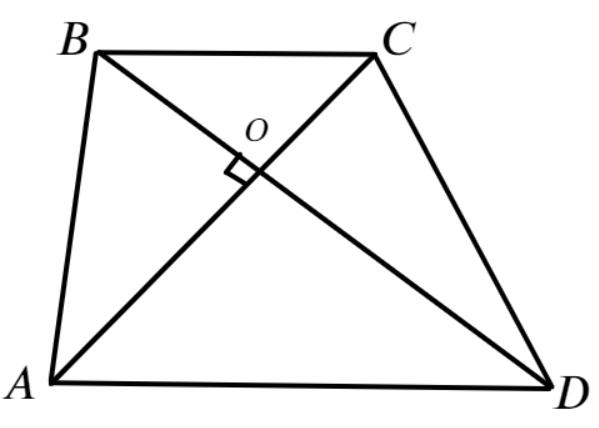
\includegraphics[scale=0.35]{g8-115.png}}
\end{figure}\\
Треугольники $AOB,\ BOC,\ COD$ и $AOD$ являются прямоугольными. Пусть $AO=x,\ CO=6-x,\ BO=y,\ DO=7-y.$ Тогда $S_{ABCD}=S_{\Delta AOB}+S_{\Delta BOC}+S_{\Delta COD}+S_{\Delta AOD}=\cfrac{xy}{2}+\cfrac{y(6-x)}{2}+\cfrac{(6-x)(7-y)}{2}+\cfrac{x(7-y)}{2}=\cfrac{xy+6y-xy+42-6y-7x+xy+7x-xy}{2}=21.$\\
